\documentclass[12pt,a4paper]{report}

% Base: student-supplied report template. Layout and front matter are retained,
% with compile-safe logo placeholders where the original image files are absent.
\usepackage{newtxtext,newtxmath}
\usepackage[T1]{fontenc}
\usepackage[utf8]{inputenc}
\usepackage{graphicx}
\usepackage{setspace}
\usepackage{geometry}
\usepackage{fancyhdr}
\usepackage{array,tabularx,ragged2e,booktabs,longtable}
\usepackage{titlesec,tocloft,float}
\usepackage{amsfonts}
\usepackage{tikz}
\usetikzlibrary{arrows.meta,positioning,shapes.geometric,fit,calc}
\usepackage{hyperref}
\usepackage[numbers,sort&compress]{natbib}

\geometry{a4paper,left=1.25in,right=0.75in,top=0.85in,bottom=0.8in,headheight=14pt,headsep=0.18in}
\setstretch{1.5}
\setlength{\parindent}{0.45in}
\setlength{\parskip}{0pt}
\setlength{\emergencystretch}{2em}
\AtBeginDocument{\justifying}
\hypersetup{colorlinks=true,linkcolor=black,citecolor=black,urlcolor=blue,pdftitle={Karavali-Transit Mini-Project Report},pdfauthor={Manushri P M, Prakruthi V Patkar, Sanath, Vamshi K}}

\titleformat{\chapter}[display]{\normalfont\bfseries\centering\fontsize{16}{19}\selectfont}{\MakeUppercase{\chaptertitlename}\ \thechapter}{8pt}{\fontsize{16}{19}\selectfont}
\titlespacing*{\chapter}{0pt}{-10pt}{18pt}
\titleformat{\section}{\normalfont\bfseries\fontsize{14}{17}\selectfont}{\thesection}{1em}{}
\titleformat{\subsection}{\normalfont\bfseries\fontsize{12}{15}\selectfont}{\thesubsection}{1em}{}
\titlespacing*{\section}{0pt}{16pt}{7pt}
\titlespacing*{\subsection}{0pt}{12pt}{5pt}
\setcounter{tocdepth}{2}
\renewcommand{\contentsname}{TABLE OF CONTENTS}
\renewcommand{\arraystretch}{1.18}

\pagestyle{fancy}\fancyhf{}
\lhead{\fontsize{9}{11}\selectfont Karavali-Transit}
\rhead{\fontsize{9}{11}\selectfont Chapter \thechapter}
\lfoot{\fontsize{8}{10}\selectfont Department of Information Science \& Engineering, SCEM, Mangaluru}
\rfoot{\fontsize{9}{11}\selectfont Page \thepage}
\renewcommand{\headrulewidth}{0.4pt}\renewcommand{\footrulewidth}{0.4pt}
\fancypagestyle{plain}{\fancyhf{}\lfoot{\fontsize{8}{10}\selectfont Department of Information Science \& Engineering, SCEM, Mangaluru}\rfoot{\fontsize{9}{11}\selectfont Page \thepage}\renewcommand{\headrulewidth}{0pt}\renewcommand{\footrulewidth}{0.4pt}}

\newcommand{\projecttitle}{Karavali-Transit: A Real-Time GPS-Enabled Intelligent Transit Monitoring and Passenger Assistance Platform}
\newcommand{\academicyear}{2026--27}
\newcommand{\logoimage}[2]{\IfFileExists{#1}{\includegraphics[width=#2,keepaspectratio]{#1}}{\fbox{\parbox[c][0.72in][c]{#2}{\centering\small Logo file not supplied\\\texttt{#1}}}}}
\newcommand{\placeholder}[1]{\fbox{\parbox{0.91\linewidth}{\centering\small\textit{Screenshot placeholder: #1. Replace with a project screenshot before final submission.}}}}
\newcommand{\implemented}{\textbf{Implemented: }}
\newcommand{\future}{\textbf{Future scope: }}

\tikzset{block/.style={draw=blue!55!black,rounded corners=3pt,fill=blue!5,align=center,text width=2.45cm,minimum height=0.85cm,font=\small},store/.style={draw=green!50!black,cylinder,shape border rotate=90,aspect=0.25,fill=green!6,align=center,minimum height=1cm,text width=2cm,font=\small},actor/.style={draw=gray!70,rounded corners=3pt,fill=gray!5,align=center,text width=2.2cm,minimum height=0.8cm,font=\small},arrow/.style={-{Stealth[length=2mm]},thick,draw=blue!65!black},dashedarrow/.style={-{Stealth[length=2mm]},thick,dashed,draw=gray!75}}

\begin{document}

% Cover page from the supplied template, with corrected scale and spacing.
\begin{titlepage}\thispagestyle{empty}\centering
{\large\bfseries VISVESVARAYA TECHNOLOGICAL UNIVERSITY}\\
{\large\bfseries ``JNANA SANGAMA'', BELAGAVI -- 590 018}
\vspace{0.10in}

\logoimage{vtu logo.jpeg}{0.85in}

\vspace{0.08in}
{\large\bfseries A MINI-PROJECT REPORT}\\\textbf{on}
\vspace{0.12in}

{\Large\bfseries ``\projecttitle''}

\vspace{0.18in}{\normalsize\textit{\bfseries Submitted by}}
\vspace{0.10in}

\begin{tabular}{@{}p{3.35in}p{1.45in}@{}}
\textbf{Manushri P M} & \textbf{4SF24IS054}\\[3pt]
\textbf{Prakruthi V Patkar} & \textbf{4SF24IS070}\\[3pt]
\textbf{Sanath} & \textbf{4SF24IS092}\\[3pt]
\textbf{Vamshi K} & \textbf{4SF24IS119}
\end{tabular}

\vspace{0.10in}{\small\textit{In partial fulfillment of the requirements for the V Semester of}}
\vspace{0.04in}{\large\bfseries BACHELOR OF ENGINEERING}\\{\bfseries in}\\{\large\bfseries INFORMATION SCIENCE \& ENGINEERING}
\vspace{0.08in}{\small\textit{Under the Guidance of}}\\[2pt]
{\bfseries Dr. Suchetha G}\\{\small Designation to be confirmed, Department of ISE}
\vspace{0.10in}

\logoimage{Sayhadri.jpg}{1.0in}

\vspace{0.03in}{\Large\bfseries SAHYADRI}\\{\large\bfseries College of Engineering \& Management}\\{\normalsize\bfseries An Autonomous Institution}\\{\normalsize\bfseries Adyar, Mangaluru -- 575 007}
\vspace{0.08in}{\large\bfseries AY: \academicyear}
\end{titlepage}

\pagenumbering{roman}\setcounter{page}{1}\pagestyle{plain}
\begin{center}
{\LARGE\bfseries SAHYADRI}\\{\Large\bfseries College of Engineering \& Management}\\{\large\bfseries An Autonomous Institution}\\Adyar, Mangaluru -- 575 007
\vspace{0.12in}\\{\large\bfseries Department of Information Science \& Engineering}\\[0.10in]
\logoimage{Sayhadri.jpg}{1.05in}\\[0.08in]{\Large\bfseries CERTIFICATE}
\end{center}
\vspace{0.12in}

\noindent This is to certify that the Mini-Project Work (IS522P7I) entitled \textbf{``\projecttitle''} has been carried out by \textbf{Manushri P M (4SF24IS054), Prakruthi V Patkar (4SF24IS070), Sanath (4SF24IS092) and Vamshi K (4SF24IS119)}, bonafide students of Sahyadri College of Engineering \& Management, in partial fulfillment of the requirements for the V Semester of Bachelor of Engineering in Information Science \& Engineering (ISE) of Visvesvaraya Technological University, Belagavi, during the Academic Year \academicyear.

It is certified that corrections or suggestions indicated for the Continuous Internal Assessment have been incorporated in the report deposited in the library of the ISE department. The mini-project report has been approved as it satisfies the academic requirements in respect of mini-project work prescribed for the said degree.

\vspace{0.35in}
\begin{center}
\begin{tabularx}{\textwidth}{>{\centering\arraybackslash}X>{\centering\arraybackslash}X>{\centering\arraybackslash}X}
\rule{1.45in}{0.4pt}&\rule{1.45in}{0.4pt}&\rule{1.45in}{0.4pt}\\[5pt]
\textbf{Dr. Suchetha G}&\textbf{Mini-Project Coordinator}&\textbf{HoD}\\[4pt]
Guide name/\newline designation to confirm&Ms. Sneha Bose&Dr. Rithesh Pakkala P.\\
Department of ISE, SCEM&Assistant Professor, Dept. of ISE&Associate Professor, ISE \& CSE (DS)
\end{tabularx}
\end{center}

\clearpage
\begin{center}{\LARGE\bfseries SAHYADRI}\\{\Large\bfseries College of Engineering \& Management}\\{\large\bfseries An Autonomous Institution}\\Adyar, Mangaluru -- 575 007\\[0.10in]{\large\bfseries Department of Information Science \& Engineering}\\[0.08in]\logoimage{Sayhadri.jpg}{1.05in}\\[0.08in]{\Large\bfseries DECLARATION}\end{center}
\vspace{0.12in}

\noindent We hereby declare that the work embodied in this Mini-Project Work (IS522P7I) Report titled \textbf{``\projecttitle''} has been carried out by us at Sahyadri College of Engineering \& Management, Mangaluru, under the supervision of \textbf{Dr. Suchetha G}, for the requirements of V Semester of Bachelor of Engineering in Information Science \& Engineering. This report has not been submitted to this or any other university for the award of any other degree.

\vspace{0.35in}\begin{flushright}
\textbf{Manushri P M (4SF24IS054)}\\\textbf{Prakruthi V Patkar (4SF24IS070)}\\\textbf{Sanath (4SF24IS092)}\\\textbf{Vamshi K (4SF24IS119)}\\Department of ISE, SCEM, Mangaluru
\end{flushright}

\clearpage
\chapter*{ABSTRACT}\addcontentsline{toc}{chapter}{Abstract}
Karavali-Transit is a web application for passenger information, bus-fleet administration, and conductor-assisted location reporting along the Mangaluru--Kundapura coastal corridor. The implementation combines a React single-page interface with an Express API, Socket.IO event delivery, and a relational database that can run on SQLite or, when configured, PostgreSQL. Passengers can search journeys by boarding and destination stops, inspect bus schedules and route timelines, and open a map view for available live vehicle positions. Fleet owners can authenticate by email one-time password (OTP), maintain buses, routes, schedules and conductor assignments, and review fleet activity. Conductors authenticate through an agency verification and conductor identification flow, initialize a shift, and may start browser geolocation tracking from a mobile device.

Location updates are submitted to the backend, checked for session, assigned vehicle and coordinate plausibility, written to telemetry storage, and broadcast to connected clients. The user interface distinguishes live tracking from states such as not tracking or offline. The report describes the repository implementation as inspected; it does not claim integration with an external transit feed, automated traffic-aware ETA, payment, ticket booking, or production email OTP delivery. Four existing code test files covering twelve utility and authentication assertions passed during preparation. The application build and report compilation are recorded separately in Chapter 8. The resulting project demonstrates a small end-to-end web architecture for corridor-based passenger information and fleet operations, while leaving deployment, real email delivery, privacy governance, and wider field validation as future work.

\clearpage
\chapter*{ACKNOWLEDGEMENT}\addcontentsline{toc}{chapter}{Acknowledgement}
We express our sincere gratitude to our guide, \textbf{Dr. Suchetha G}, Department of Information Science \& Engineering, for advice and encouragement during this mini-project.

We thank \textbf{Ms. Sneha Bose}, Mini-Project Coordinator, and the project coordinators of the Department of Information Science \& Engineering for their support. We are grateful to \textbf{Dr. Rithesh Pakkala P.}, Head of the Department, for his guidance and encouragement. We also thank the faculty and staff of Sahyadri College of Engineering \& Management, our families and friends, for their support.

\vspace{0.2in}\begin{flushright}\textbf{Manushri P M (4SF24IS054)}\\\textbf{Prakruthi V Patkar (4SF24IS070)}\\\textbf{Sanath (4SF24IS092)}\\\textbf{Vamshi K (4SF24IS119)}\end{flushright}

\clearpage\tableofcontents
\clearpage\listoffigures
\clearpage\listoftables
\clearpage\pagenumbering{arabic}\setcounter{page}{1}\pagestyle{fancy}

% -----------------------------------------------------------------------------
\chapter{Introduction}
\section{Background}
Public transport users make decisions before and during a journey: where to board, which service to take, and whether a vehicle is approaching. Smaller private-bus corridors may not expose one integrated digital source for schedules, operator details, and vehicle position. Karavali-Transit addresses this information problem for a fixed coastal Karnataka corridor by placing passenger search, fleet administration, conductor operations, and location sharing in one browser-accessible system.

The application models nine corridor stops in a fixed order: Mangaluru, Kuntikana, Kulur, Surathkal, Mulki, Padubidri, Kaup, Udupi, and Kundapura. Stop aliases, Kannada names, localities, landmarks, and coordinates are maintained in project data. Journey search checks that the chosen origin precedes the destination along a bus's ordered stops. This is a corridor-specific system rather than a general national journey planner.

\section{Purpose and Scope}
The purpose is to demonstrate how stored bus and timetable data can be combined with optional phone geolocation to provide route discovery and live location information. The system has three user areas: a public passenger portal, an authenticated fleet-owner portal, and a conductor terminal. The passenger portal does not require passenger account creation. Owner functions include bus and conductor management; conductor functions include agency verification, conductor lookup or registration, shift initialization, and tracking control.

Scope is limited to the features represented in the current source code and database layer. Bus search, route details, maps, feedback, fleet management, authentication flows, shifts, telemetry and Socket.IO updates are included. Real external OTP delivery, deployment-grade operations, payment and ticket issuance, certified arrival-time prediction, and integration with government or GTFS feeds are outside the implementation described here.

\section{Project Overview}
The frontend is a React application built with Vite. It calls JSON endpoints served by Express and receives changes through Socket.IO. Leaflet and React-Leaflet render map views. The database module supplies SQLite as the default store and includes a PostgreSQL path selected through configuration. The conductor browser obtains location only after the tracking action and browser permission; the coordinates are sent to the server and then made available to passenger clients.

\section{Organization of the Report}
Chapter 2 reviews transit information and location technology. Chapters 3 and 4 formulate the problem and specify requirements. Chapter 5 explains the design and workflows; Chapter 6 maps those designs to the repository implementation. Chapter 7 presents test design and observed code-level test results. Chapter 8 discusses application outcomes and limitations, and Chapter 9 concludes with future work.

% -----------------------------------------------------------------------------
\chapter{Literature Survey}
\section{Passenger Information and Vehicle Location}
Passenger information systems communicate service schedules, disruptions, vehicle position, and arrival estimates. A review by Brakewood and Watkins examined reported passenger benefits of real-time transit information and found outcomes related to passenger waiting and travel experience, while noting that the effect depends on context and the information supplied \cite{brakewood2019}. This supports the project's focus on making route and vehicle information accessible to passengers; it does not establish that this prototype has measured those benefits.

Automatic vehicle location systems combine a positioning source with communications and an information service. A smartphone can provide a practical location source when a dedicated onboard tracking unit is unavailable. The browser Geolocation API exposes coordinates and related measurements only subject to browser support, secure-context rules, and user permission \cite{w3cgeo}. Thus the application treats the conductor's phone as the GPS device and reports errors when location cannot be obtained.

\section{Real-Time Data Exchange}
GTFS Realtime defines message concepts for vehicle positions, trip updates, and service alerts so agencies can publish real-time service data to consumers \cite{gtfsrt}. Karavali-Transit uses its own JSON API and Socket.IO events; it does not implement GTFS static or realtime feeds. The GTFS model is relevant as a reference for separating vehicle position from schedule and alert data, and as a possible future interoperability target.

Socket.IO provides event-based, bidirectional communication between a browser client and server, including broadcast patterns suitable for updating several connected views \cite{socketio}. The project emits location and tracking status events to connected clients. The server also persists a telemetry record, so live delivery and history have separate roles.

\section{Web Maps and Application Frameworks}
Leaflet is a JavaScript library for interactive maps and supplies the map primitives used through React-Leaflet in the passenger view \cite{leaflet}. React structures the user interface as stateful components; Express supplies HTTP routing and middleware for the backend \cite{react,express}. These frameworks provide implementation building blocks, while route-order matching, role workflows, validation and the coastal stop data are project-specific.

\section{Comparison and Project Position}
Many transit platforms rely on operator feeds, dedicated AVL devices, or multimodal datasets. The present prototype instead centers on a defined route, manually administered bus schedules, and conductor phone location. It demonstrates the data path end to end, but does not claim the coverage, prediction accuracy, service availability, or feed interoperability of a deployed agency system. The gap addressed is a compact, maintainable corridor prototype that connects basic operator-maintained information to a passenger-facing search and map.

% -----------------------------------------------------------------------------
\chapter{Problem Formulation and Objectives}
\section{Problem Statement}
Passengers on the selected coastal corridor need to identify buses serving a stop-to-stop journey and to see a vehicle's reported location when a conductor is actively sharing it. Fleet operators need a way to maintain bus particulars, schedules, route stops, and conductor assignments. Without a single connected interface, route information and current operational state can be separated across informal channels. The project formulates the problem as building a web application that stores corridor and fleet data, supports role-specific workflows, and shares validated location updates with public clients.

\section{Objectives}
\begin{enumerate}
\item Provide a public interface to search buses between ordered corridor stops.
\item Show bus details and a stop-by-stop planned timetable, with a map view for live location when available.
\item Provide owner authentication and tools to administer buses, stops, schedules and conductors.
\item Allow a conductor to authenticate, initialize duty, and explicitly start or stop phone-based location tracking.
\item Validate incoming location data and distribute changes to connected passenger views.
\item Keep durable bus, route, shift, feedback and telemetry records in a relational store.
\end{enumerate}

\section{Existing Approach and Proposed System}
The project repository does not document a measured baseline process, so no quantitative claim about a previous manual system is made. The proposed system provides a single application with public and authenticated portals. Search and route details use stored route/timetable data; location is available only when tracking is started and valid updates are received. This is a prototype design and its results should be interpreted within the configured sample data and runtime environment.

\section{Assumptions and Constraints}
The route order and bus stop times are entered or seeded by the application. The conductor uses a compatible browser and grants location permission. Browser geolocation generally requires a secure context in deployment. Network coverage affects update delivery. OTP codes are held in process memory in the inspected source; owner OTP delivery explicitly reports unavailable in production configuration, while development exposes a preview code. These are implementation constraints and are not presented as production-ready identity delivery.

% -----------------------------------------------------------------------------
\chapter{System Requirements}
\section{Functional Requirements}
\begin{longtable}{p{0.12\textwidth}p{0.78\textwidth}}
\toprule\textbf{ID}&\textbf{Requirement}\\\midrule
FR-01&The public portal shall allow a passenger to select origin and destination stops and search matching buses.\\
FR-02&The public portal shall display bus particulars, service type, planned schedule and ordered route details.\\
FR-03&The public portal shall display live tracking state and map position when valid location data is available.\\
FR-04&An owner shall authenticate with an email OTP before accessing protected fleet functions.\\
FR-05&An authenticated owner shall add, view, edit and delete fleet buses and manage route stops and schedules.\\
FR-06&An owner shall manage conductor records/assignments and view fleet dashboard or activity information.\\
FR-07&A conductor shall verify the agency, identify or register their conductor record, and initialize duty for a bus.\\
FR-08&A conductor shall explicitly start and stop browser location tracking during a shift.\\
FR-09&The backend shall validate submitted coordinates and bind protected telemetry to the conductor session and assigned bus.\\
FR-10&The system shall record feedback and operational records supported by its database/API.\\
\bottomrule
\end{longtable}

\section{Non-Functional Requirements}
The interface should be usable from a desktop or mobile browser and should communicate tracking state clearly. The backend should reject malformed or implausible location reports and protect owner and conductor operations with session checks where implemented. Database access should be isolated behind a module that supports the configured SQL engine. Network-dependent functions should fail visibly when unavailable. Location is personal data; it should be collected only for the tracking task and should receive appropriate notice, access control, retention and transport protection before production deployment, consistent with geolocation privacy guidance \cite{w3cgeo}.

\section{Software Requirements}
\begin{table}[H]\centering\small\caption{Software stack evidenced by the repository}\label{tab:stack}
\begin{tabularx}{\textwidth}{p{0.25\textwidth}X}\toprule\textbf{Layer}&\textbf{Implementation}\\\midrule
Client&React 19, Vite 8, Tailwind CSS, Lucide icons\\
Mapping&Leaflet 1.9 and React-Leaflet 5\\
Server&Node.js ES modules, Express 5, Socket.IO 4\\
Database&SQLite through sqlite3 by default; PostgreSQL through pg when USE\_POSTGRES=true\\
Validation and tests&Node.js native test runner (node:test), Oxlint\\
\bottomrule\end{tabularx}\end{table}

Exact runtime version used by the project authors was not supplied. The package manifest describes dependency ranges; the local installation used for this report compiled under its available Node.js runtime. Production hosting, TLS termination, SMTP provider, backup schedule, and deployment environment remain to be specified.

\section{Hardware Requirements}
No dedicated GPS hardware is required by the current design. A conductor needs a phone or other browser-enabled device with a location provider and network connection. Passenger and owner users need an internet-connected device with a modern browser. A server host must be able to run Node.js and access the selected SQL database. Capacity and minimum device specifications have not been benchmarked and are not prescribed as measured values.

% -----------------------------------------------------------------------------
\chapter{System Design and Methodology}
\section{System Architecture}
The frontend separates the passenger, owner and conductor experiences. The API handles HTTP operations and session checks, while Socket.IO relays real-time updates. The data module abstracts SQLite/PostgreSQL persistence. Static corridor and UI data coexist with relational bus, stop, shift and telemetry data.

\begin{figure}[tbp]\centering
\resizebox{0.98\textwidth}{!}{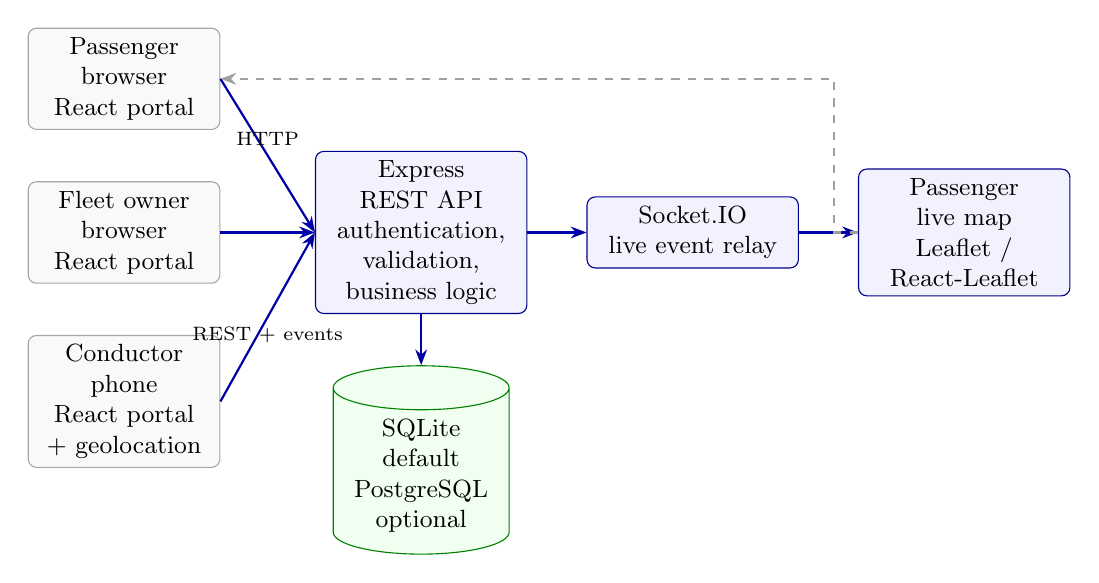
\begin{tikzpicture}[node distance=0.65cm and 0.75cm]
\node[actor] (pass) {Passenger browser\\React portal};
\node[actor,below=of pass] (owner) {Fleet owner browser\\React portal};
\node[actor,below=of owner] (cond) {Conductor phone\\React portal + geolocation};
\node[block,right=1.2cm of owner] (api) {Express REST API\\authentication, validation, business logic};
\node[block,right=of api] (rt) {Socket.IO\\live event relay};
\node[store,below=of api] (db) {SQLite default\\PostgreSQL optional};
\node[block,right=of rt] (map) {Passenger live map\\Leaflet / React-Leaflet};
\draw[arrow] (pass.east) -- node[above,font=\scriptsize]{HTTP} (api.west);
\draw[arrow] (owner.east) -- (api.west);
\draw[arrow] (cond.east) -- node[below,font=\scriptsize]{REST + events} (api.west);
\draw[arrow] (api) -- (db);
\draw[arrow] (api) -- (rt);
\draw[arrow] (rt) -- (map);
\draw[dashedarrow] (map.west) -- ++(-0.3,0) |- (pass.east);
\end{tikzpicture}}\caption{Karavali-Transit logical system architecture}\label{fig:architecture}\end{figure}

\section{Data Flow}
Passenger searches are request-response operations. The browser sends selected stops to a public endpoint and receives matching bus information. During tracking, the conductor browser reads location, sends the measurement to an authenticated endpoint, and the server validates and records it before broadcasting a public-safe bus payload. Clients update the map from the broadcast. The API can also supply recent persisted or current data when a client loads.

\begin{figure}[tbp]\centering
\resizebox{0.95\textwidth}{!}{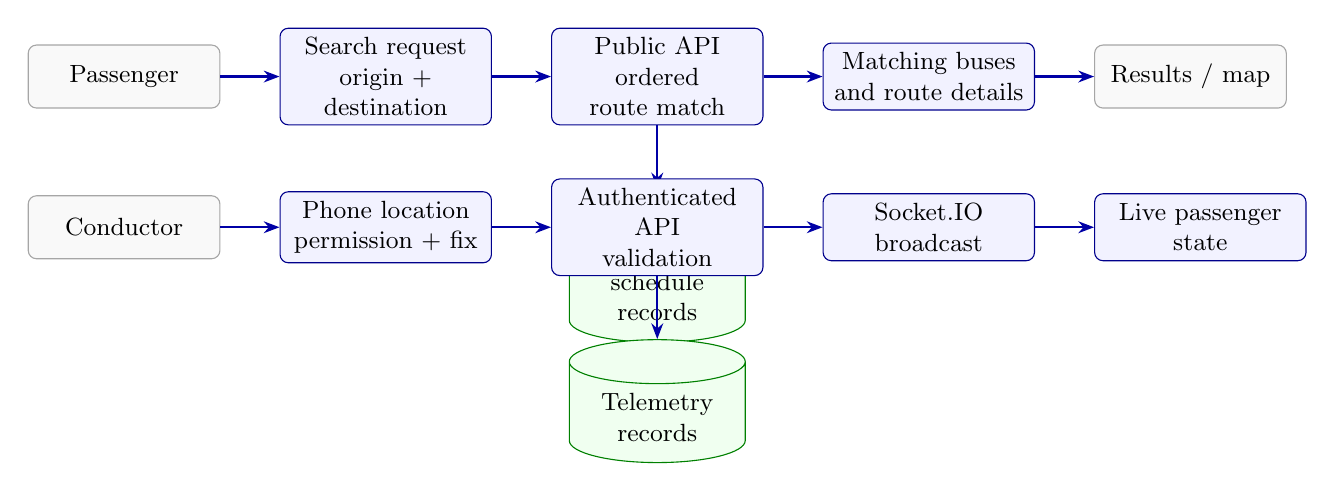
\begin{tikzpicture}[node distance=0.8cm and 0.75cm]
\node[actor] (p) {Passenger};\node[block,right=of p] (search) {Search request\\origin + destination};\node[block,right=of search] (svc) {Public API\\ordered route match};\node[store,below=of svc] (data) {Bus and stop\\schedule records};\node[block,right=of svc] (result) {Matching buses\\and route details};\node[actor,right=of result] (screen) {Results / map};
\draw[arrow] (p)--(search);\draw[arrow] (search)--(svc);\draw[arrow] (svc)--(data);\draw[arrow] (svc)--(result);\draw[arrow] (result)--(screen);
\node[actor,below=1.1cm of p] (c) {Conductor};\node[block,right=of c] (gps) {Phone location\\permission + fix};\node[block,right=of gps] (valid) {Authenticated API\\validation};\node[store,below=of valid] (tele) {Telemetry\\records};\node[block,right=of valid] (broadcast) {Socket.IO\\broadcast};\node[block,right=of broadcast] (live) {Live passenger\\state};
\draw[arrow] (c)--(gps);\draw[arrow] (gps)--(valid);\draw[arrow] (valid)--(tele);\draw[arrow] (valid)--(broadcast);\draw[arrow] (broadcast)--(live);
\end{tikzpicture}}\caption{Context-level data flow for search and live location}\label{fig:dfd}\end{figure}

\section{Use-Case Model}
The use cases are organized by role. Passenger use is public. Owner operations require an owner session. Conductor tracking requires an active conductor token and browser location permission. The diagram summarizes user interactions; it does not imply that every action requires a separate database account.

\begin{figure}[tbp]\centering
\resizebox{0.94\textwidth}{!}{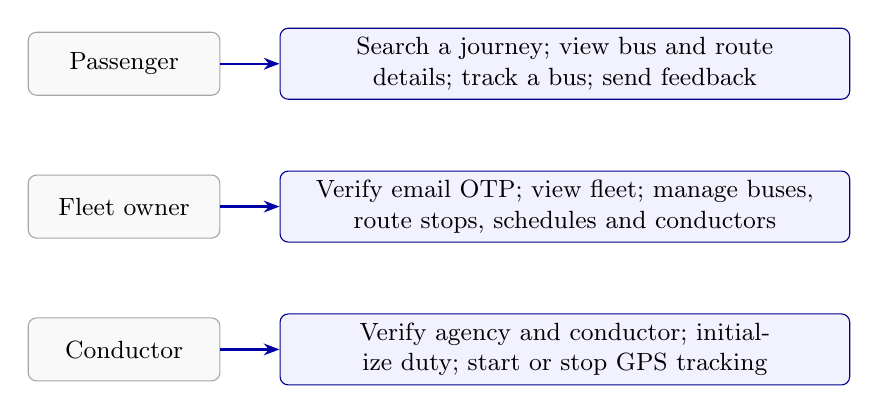
\begin{tikzpicture}[node distance=1.0cm and 0.75cm]
\node[actor] (pass) {Passenger};\node[block,right=of pass,text width=7cm] (pcases) {Search a journey; view bus and route details; track a bus; send feedback};
\node[actor,below=of pass] (owner) {Fleet owner};\node[block,right=of owner,text width=7cm] (ocases) {Verify email OTP; view fleet; manage buses, route stops, schedules and conductors};
\node[actor,below=of owner] (cond) {Conductor};\node[block,right=of cond,text width=7cm] (ccases) {Verify agency and conductor; initialize duty; start or stop GPS tracking};
\draw[arrow] (pass)--(pcases);\draw[arrow] (owner)--(ocases);\draw[arrow] (cond)--(ccases);
\end{tikzpicture}}\caption{Primary use cases by application role}\label{fig:usecase}\end{figure}

\section{Database Design}
The schema is initialized for both supported SQL engines. The following ER view shows the principal relationships from the schema definitions. Some operational state, including the active OTP cache and active bus snapshots, is held in server memory rather than a permanent table.

\begin{figure}[tbp]\centering
\resizebox{0.98\textwidth}{!}{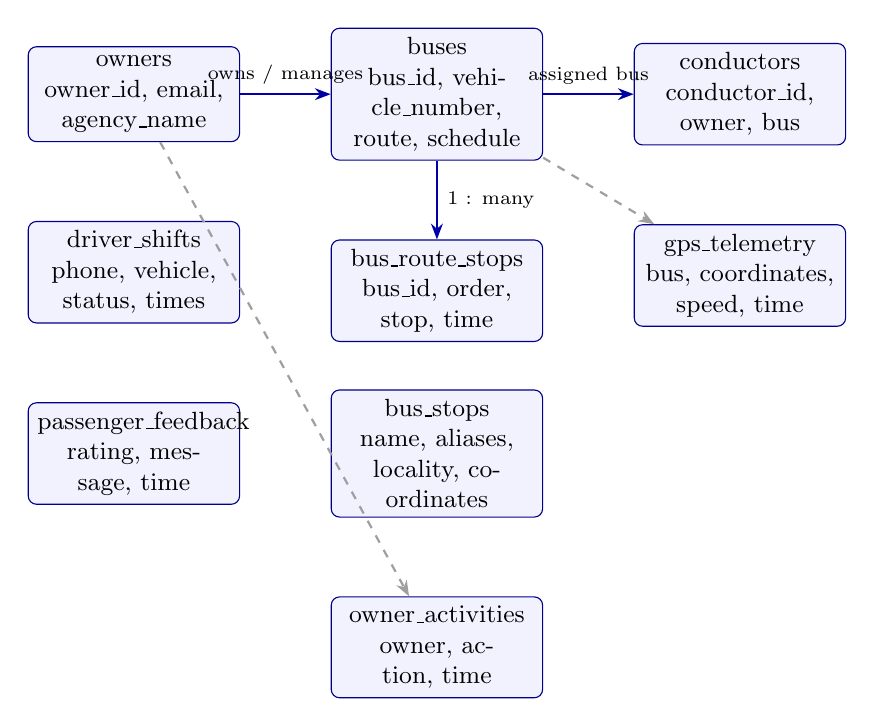
\begin{tikzpicture}[node distance=1.0cm and 1.15cm]
\node[block] (owners) {owners\\owner\_id, email, agency\_name};
\node[block,right=of owners] (buses) {buses\\bus\_id, vehicle\_number, route, schedule};
\node[block,below=of buses] (stops) {bus\_route\_stops\\bus\_id, order, stop, time};
\node[block,right=of buses] (cond) {conductors\\conductor\_id, owner, bus};
\node[block,below=of owners] (shift) {driver\_shifts\\phone, vehicle, status, times};
\node[block,below=of cond] (gps) {gps\_telemetry\\bus, coordinates, speed, time};
\node[block,below=of shift] (feedback) {passenger\_feedback\\rating, message, time};
\node[block,right=of feedback] (busstop) {bus\_stops\\name, aliases, locality, coordinates};
\node[block,below=of busstop] (activity) {owner\_activities\\owner, action, time};
\draw[arrow] (owners)--node[above,font=\scriptsize]{owns / manages}(buses);
\draw[arrow] (buses)--node[right,font=\scriptsize]{1 : many}(stops);
\draw[arrow] (buses)--node[above,font=\scriptsize]{assigned bus}(cond);
\draw[dashedarrow] (buses)--(gps);
\draw[dashedarrow] (owners)--(activity);
\end{tikzpicture}}\caption{Principal relational entities and associations}\label{fig:er}\end{figure}

The schema also includes \texttt{email\_otps}; the inspected authentication routes currently keep active OTP values in an in-memory object. Its presence in schema initialization should not be read as proof that the current flow persists OTPs there. Route stop records reference buses and cascade on bus deletion in the defined SQL schema. The design is relational, but the exact production database and retention policy depend on deployment configuration.

\section{GPS Tracking Workflow}
The conductor first initializes a shift. Starting tracking invokes \texttt{navigator.geolocation.\allowbreak watchPosition} with high accuracy requested. For each location callback, the client packages latitude, longitude, accuracy, speed, heading, timestamp and occupancy fields. The server checks the session, bus assignment, coastal bounding coordinates, accuracy, speed and timestamp; it updates in-memory current state, persists telemetry, and emits a location event. Browser permission denial or missing GPS is surfaced in the conductor UI. Stopping tracking clears the watch and calls the stop-tracking endpoint.

\begin{figure}[tbp]\centering
\resizebox{0.94\textwidth}{!}{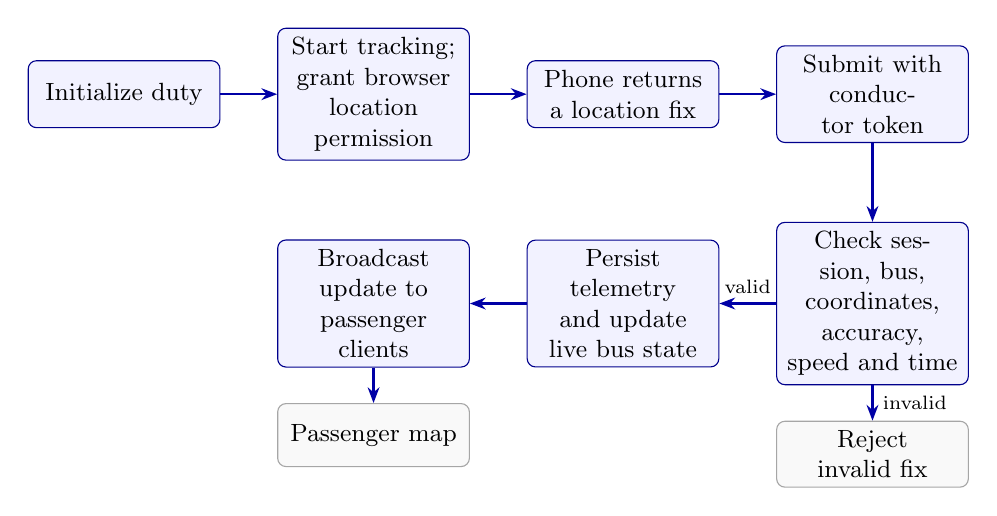
\begin{tikzpicture}[node distance=0.45cm and 0.72cm]
\node[block,text width=2.2cm] (duty) {Initialize duty};
\node[block,text width=2.2cm,right=of duty] (permission) {Start tracking; grant browser location permission};
\node[block,text width=2.2cm,right=of permission] (gps) {Phone returns a location fix};
\node[block,text width=2.2cm,right=of gps] (submit) {Submit with conductor token};
\node[block,text width=2.2cm,below=1cm of submit] (validate) {Check session, bus, coordinates, accuracy, speed and time};
\node[block,text width=2.2cm,left=of validate] (persist) {Persist telemetry and update live bus state};
\node[block,text width=2.2cm,left=of persist] (broadcast) {Broadcast update to passenger clients};
\node[actor,below=of broadcast] (map) {Passenger map};
\node[actor,below=of validate] (reject) {Reject invalid fix};
\draw[arrow] (duty)--(permission);\draw[arrow] (permission)--(gps);\draw[arrow] (gps)--(submit);\draw[arrow] (submit)--(validate);\draw[arrow] (validate)--node[above,font=\scriptsize]{valid}(persist);\draw[arrow] (persist)--(broadcast);\draw[arrow] (broadcast)--(map);\draw[arrow] (validate)--node[right,font=\scriptsize]{invalid}(reject);
\end{tikzpicture}}\caption{GPS tracking and server validation workflow}\label{fig:gps}\end{figure}

\section{Application Workflow}
At a high level, the passenger selects stops and examines matching services; an owner configures fleet records; a conductor verifies identity, selects/uses an assigned bus, initializes a shift, and optionally shares location. The live map consumes updates only when available. The separation keeps schedule information useful when no bus is currently transmitting.

\begin{figure}[tbp]\centering
\resizebox{0.95\textwidth}{!}{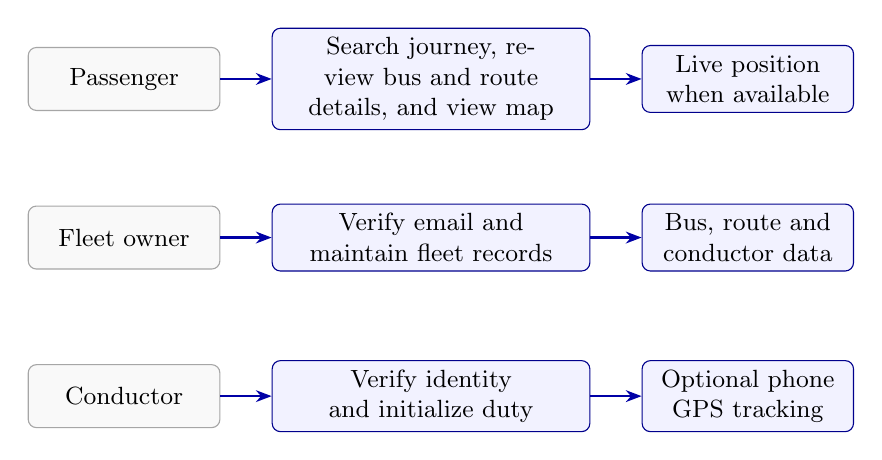
\begin{tikzpicture}[node distance=1.2cm and 0.65cm]
\node[actor] (pass) {Passenger};\node[block,text width=3.8cm,right=of pass] (pflow) {Search journey, review bus and route details, and view map};\node[block,right=of pflow] (pout) {Live position when available};
\node[actor,below=of pass] (owner) {Fleet owner};\node[block,text width=3.8cm,right=of owner] (oflow) {Verify email and maintain fleet records};\node[block,right=of oflow] (oout) {Bus, route and conductor data};
\node[actor,below=of owner] (cond) {Conductor};\node[block,text width=3.8cm,right=of cond] (cflow) {Verify identity and initialize duty};\node[block,right=of cflow] (track) {Optional phone GPS tracking};
\draw[arrow] (pass)--(pflow);\draw[arrow] (pflow)--(pout);\draw[arrow] (owner)--(oflow);\draw[arrow] (oflow)--(oout);\draw[arrow] (cond)--(cflow);\draw[arrow] (cflow)--(track);
\end{tikzpicture}}\caption{Role-based application workflow}\label{fig:workflow}\end{figure}

% -----------------------------------------------------------------------------
\chapter{Implementation}
\section{Repository Structure}
The UI is implemented in \texttt{src/}. \texttt{App.jsx} coordinates portal and passenger-screen state; \texttt{PassengerPortal.jsx}, \texttt{OwnerPortal.jsx}, and \texttt{ConductorPortal.jsx} contain the main role interfaces. Shared passenger components and map code are in \texttt{src/components/} and \texttt{TransitMap.jsx}. \texttt{server.js} defines HTTP and Socket.IO behavior, \texttt{db.js} contains schema setup and persistence helpers, and \texttt{serverAuth.js} contains session/token validation helpers. \texttt{tests/} contains Node.js test files.

\section{Passenger Portal}
The passenger UI provides autocomplete and stop selection, swaps selected stops, submits a journey request, and displays matching bus cards. The backend search route uses stored route stops and returns services that serve the requested forward journey. A details view displays vehicle information and the planned route timeline. The map is rendered with Leaflet; current location and live/offline status are derived from available bus state and server events. Public endpoints include stop search, nearby/all stops, bus journey search, bus details, route details, and location state. Passenger feedback is submitted through a public endpoint.

No seat reservation, ticket purchase or fare collection is implemented as a passenger transaction. A test file includes fare and sorting utility tests, but the active passenger API contract and screens should be described based on their actual functionality, not inferred from the presence of utility code.

\section{Fleet Owner Portal}
The owner submits an email to \path{/api/owner/send-otp}; successful verification at \path{/api/owner/verify-otp} creates a bearer session. Protected dashboard, buses, conductors and activity endpoints check the owner token. Bus registration accepts vehicle/operator, route, service type, seat capacity, timetable and ordered stops; edit and delete operations update corresponding records. Conductors are associated with an owner and may reference an assigned bus. The current My Buses interface presents View, Edit and Delete actions. Details are selected on demand and closed through the panel close control.

\section{Conductor Portal and Tracking}
The conductor flow verifies an agency email OTP, then looks up a conductor by agency and mobile number or allows registration. It stores a conductor token in browser local storage. Duty initialization posts bus and conductor details to \path{/api/conductor/start-duty}. Tracking is a separate action: browser geolocation is requested only when tracking starts, and location errors update the UI. The API checks token and bus assignment and rejects values outside configured limits. Valid data is added to active bus state, persisted using the telemetry helper, and broadcast through Socket.IO events. A stop-tracking request marks the bus as no longer live.

\begin{table}[tbp]\centering\small\caption{Selected API operations in the current backend (paths are prefixed by /api)}\label{tab:api}
\begin{tabularx}{\textwidth}{p{0.12\textwidth}>{\RaggedRight\arraybackslash}p{0.34\textwidth}X}\toprule\textbf{Method}&\textbf{Endpoint}&\textbf{Purpose}\\\midrule
POST&\path{owner/send-otp}&Owner email verification request\\
POST&\path{owner/verify-otp}&Owner session creation\\
GET&\path{owner/buses}&List protected fleet buses\\
POST&\path{owner/buses}&Create a fleet bus\\
PUT&\path{owner/buses/:busId}&Edit bus information\\
DELETE&\path{owner/buses/:busId}&Delete a bus\\
POST&\path{conductor/send-otp}&Agency verification request\\
POST&\path{conductor/verify-otp}&Agency verification and session\\
POST&\path{conductor/lookup}&Find a conductor record\\
POST&\path{conductor/register}&Register a conductor\\
POST&\path{conductor/start-duty}&Initialize a conductor shift\\
POST&\path{conductor/gps-location}&Authenticated location submission and persistence\\
POST&\path{conductor/stop-tracking}&Stop tracking and broadcast offline status\\
GET&\path{public/stops/search}&Public stop discovery\\
GET&\path{public/buses/search}&Public journey search\\
GET&\path{public/buses/:id/route}&Public route details\\
GET&\path{public/buses/:id/location}&Public tracking information\\
\bottomrule\end{tabularx}\end{table}

\section{Security and Data Handling Notes}
The owner middleware requires an owner bearer session; the conductor GPS endpoint requires a conductor bearer token and verifies assigned bus consistency. Input bounds and speed/accuracy/timestamp checks are implemented for telemetry. OTP state and active session managers are in memory, so process restart clears those states. The inspected project uses CORS middleware, but the repository alone does not demonstrate a production deployment's TLS, secret management, rate limiting, audit policy, or mail transport. These should be addressed before deployment with real users.

\section{Core Processing Outline}
\begin{verbatim}
Passenger journey search:
  receive origin and destination
  resolve normalized stop names and aliases
  retrieve buses and ordered route stops
  keep buses where origin occurs before destination
  return public bus data without private owner/PIN fields

Conductor location update:
  authenticate bearer token
  verify conductor is assigned to bus
  validate coordinate, accuracy, speed and timestamp
  update current in-memory bus state
  persist telemetry record
  broadcast public-safe location event
\end{verbatim}

% -----------------------------------------------------------------------------
\chapter{Testing}
\section{Testing Approach}
The repository includes unit tests using the Node.js native test runner and integration-oriented files for the owner, conductor, GPS, and passenger flows. Tests in the current report were selected to avoid mutating the project's local SQLite database. The tests exercise pure utilities and server-auth helper behavior. The source also contains broader integration suites, but those were not executed for this report and are therefore not reported as passing.

\section{Executed Test Results}
The four suites listed below were run successfully with the Node.js native test runner, using \texttt{node --test} and explicit file arguments.

\begin{table}[H]\centering\small\caption{Observed results from the selected code tests}\label{tab:testresults}
\begin{tabularx}{\textwidth}{p{0.29\textwidth}X r}\toprule\textbf{Suite}&\textbf{Coverage represented in source}&\textbf{Result}\\\midrule
owner-auth&OTP validity/expiry/attempt limit, random owner session token and expiry, conductor PIN match, removal of PIN from public bus payload&4 passed\\
transit-utils&Destination matching behavior, including direction-aware route matching&1 passed\\
journey&Distance, destination filtering and delay status utility behavior&3 passed\\
fare-and-sort&Fare estimation utility and ETA/fare/seat sorting helpers&4 passed\\
\midrule\textbf{Total}&Selected unit-level checks&\textbf{12 passed, 0 failed}\\\bottomrule\end{tabularx}\end{table}

These results are limited to the listed tests. They do not constitute a full end-to-end verification of live OTP delivery, browser geolocation permissions, mobile map behavior, database switching, deployment security, or production load.

\section{Test Case Design}
\begin{longtable}{>{\RaggedRight\arraybackslash}p{0.08\textwidth}>{\RaggedRight\arraybackslash}p{0.25\textwidth}>{\RaggedRight\arraybackslash}p{0.33\textwidth}>{\RaggedRight\arraybackslash}p{0.19\textwidth}}
\toprule\textbf{ID}&\textbf{Test}&\textbf{Expected behavior}&\textbf{Status}\\\midrule
TC-01&Submit matching, unexpired owner OTP&Validation succeeds&Passed in selected suite\\
TC-02&Submit incorrect, expired, or attempt-limited OTP&Validation fails&Passed in selected suite\\
TC-03&Create owner session token&Token is unique and expires at configured lifetime&Passed in selected suite\\
TC-04&Filter destination against forward route&Matching direction is accepted; wrong direction is rejected&Passed in selected suite\\
TC-05&Estimate distance and classify delay&Utility returns expected calculated/classified result&Passed in selected suite\\
TC-06&Sort services by ETA, fare or seats&Ordering follows selected criterion&Passed in selected suite\\
TC-07&Submit GPS without valid conductor token&API rejects with unauthorized response&Integration test exists; not run for this report\\
TC-08&Submit coordinates outside corridor bounds&API rejects the location&Integration test exists; not run for this report\\
TC-09&Search a forward journey and inspect stop timeline&Matching bus and ordered route are returned&Integration test exists; not run for this report\\
TC-10&Exercise real browser permission and map updates&Position and map update when permission/network allow&Manual device test not recorded\\
\bottomrule
\end{longtable}

% -----------------------------------------------------------------------------
\chapter{Results and Discussion}
\section{Implemented Outcomes}
The repository provides three connected role areas. Passengers can search a journey, review matching vehicles and route timings, and view a map with a live state when current conductor telemetry is available. Owners can access a protected fleet dashboard and manage buses and conductors. Conductors can complete agency/conductor identification, initialize duty, and explicitly enable location reporting from a browser. The backend stores relevant data and relays location events to clients.

The selected 12 unit-level assertions passed. The production build completed successfully and produced the Vite output; Vite also reported that the minified JavaScript chunk exceeds its 500 kB advisory threshold. The report PDF compiled to A4 pages and was visually reviewed. These are functional and build observations, not field measurements. No measured reduction in wait time, GPS accuracy study, load test, or user satisfaction survey was present in the repository or conducted for this report.

\section{Screenshots to Insert}
The supplied LaTeX text does not include screenshots, and the repository contains no authenticated portal screenshots intended for this report. The following compact boxes identify appropriate insertion points. Replace each with a current application capture before final college submission.
\begin{figure}[tbp]\centering\small
\begin{tabularx}{\textwidth}{XX}
{\centering\textbf{(a) Passenger search and results}\par\vspace{3pt}\placeholder{Insert passenger search and bus results screenshot}\par} &
{\centering\textbf{(b) Passenger details and tracking}\par\vspace{3pt}\placeholder{Insert route details and live map screenshot}\par}\\[8pt]
{\centering\textbf{(c) Fleet owner bus management}\par\vspace{3pt}\placeholder{Insert My Buses table screenshot}\par} &
{\centering\textbf{(d) Conductor duty interface}\par\vspace{3pt}\placeholder{Insert conductor duty screenshot}\par}
\end{tabularx}
\caption{Application views to be captured from the running project}\end{figure}

\section{Limitations}
The present system is scoped to a predefined corridor and project-maintained bus data. Position freshness depends on the conductor device, permission and network. Current OTP delivery is not production-ready: the owner route disables sending in production when email delivery is unconfigured, and both OTP/session state are process-memory based. The code does not supply measured prediction accuracy or a field-tested reliability result. The availability of live positions must therefore be communicated as conditional rather than guaranteed.

% -----------------------------------------------------------------------------
\chapter{Conclusion and Future Scope}
\section{Conclusion}
Karavali-Transit brings together passenger journey search, operator fleet administration, conductor shift operations, and phone-based location sharing for a nine-stop coastal bus corridor. Its architecture combines React and Vite, Express APIs, Socket.IO live events, Leaflet mapping, and a SQLite/PostgreSQL persistence layer. A conductor location report passes through session and plausibility validation before it is stored and broadcast. This gives the prototype a clear end-to-end path from mobile location capture to passenger map display.

Selected unit-level tests passed during report preparation. However, the work remains a corridor prototype; production delivery, live field testing, privacy operations and wider reliability validation remain open tasks. The report distinguishes current repository behavior from recommended future work.

\section{Future Scope}
\begin{enumerate}
\item Configure a verified email/SMS OTP provider, persistent expiring OTP records, rate limits, and explicit session revocation/logout endpoints.
\item Deploy behind HTTPS, restrict CORS, protect credentials, define backup and telemetry retention policies, and document user consent for location sharing.
\item Conduct supervised field trials across devices and network conditions; record position freshness, coordinate error, API availability and user feedback.
\item Add schedule-aware arrival prediction only after collecting and validating sufficient time-series observations. A timetable estimate should be labeled distinctly from a validated prediction.
\item Consider importing/exporting GTFS and GTFS Realtime data for interoperability after the existing route and identifier model is mapped to that standard.
\item Add accessibility review, Kannada language coverage across all portal flows, and deployment monitoring.
\end{enumerate}

% -----------------------------------------------------------------------------
\clearpage\renewcommand{\bibname}{REFERENCES}
\bibliographystyle{unsrt}
\bibliography{references}

\end{document}
